% book example for classicthesis.sty
\documentclass[
  % Replace twoside with oneside if you are printing your thesis on a single side
  % of the paper, or for viewing on screen.
  %oneside,
  twoside,
  11pt, a4paper,
  footinclude=true,
  headinclude=true,
  cleardoublepage=empty
]{scrbook}

\usepackage{lipsum}
\usepackage[linedheaders,parts,pdfspacing]{classicthesis}
\usepackage{amsmath}
\usepackage{amsthm}
\usepackage{acronym}
\usepackage{graphicx}

\title{Measurement uncertainties in x-ray computed tomography}
\author{Joshua Greenhalgh}

\begin{document}

\maketitle

%*******************************************************
% Abstract
%*******************************************************
\pdfbookmark[1]{Abstract}{Abstract}
\chapter*{Abstract}

X-ray computed tomography (XCT) is beginning to find a range of new industrial applications. For many years this technique has been applied to non-destructive testing (NDT), however it is now being used by industry for the purpose of metrology. XCT has certain advantages over the traditional approach to metrology that of the coordinate measuring machine (CMM). Foremost among these is the ability to measure both external and internal aspects of an objects geometry without the need to destroy the object. This technique does however suffer from the lack of a clear understanding of the processes metrological uncertainties - if XCT is to be adopted more widely then it is necessary to be able to quantify the underlying uncertainties in this measuring procedure. This Thesis will approach the problem of quantifying these uncertainties via the simulation of an XCT system. The focus will be on the effect of magnification on measurement uncertainty in the presence of realistically modeled source and detector elements.

\textbf{\textit{A previous version of parts of this text was submitted as part of FEEG6018}}

The code used in this project can be found in the code directory of the GitHub repository found at https://github.com/josh-gree/thesis

%*******************************************************
% Table of Contents
%*******************************************************
\pdfbookmark[1]{\contentsname}{tableofcontents}

\setcounter{tocdepth}{2} % <-- 2 includes up to subsections in the ToC
\setcounter{secnumdepth}{3} % <-- 3 numbers up to subsubsections

\tableofcontents

%*******************************************************
% List of Figures and of the Tables
%*******************************************************

%*******************************************************
% List of Figures
%*******************************************************
\pdfbookmark[1]{\listfigurename}{lof}
\listoffigures

%*******************************************************
% List of Tables
%*******************************************************
\pdfbookmark[1]{\listtablename}{lot}
\listoftables
  



\chapter{Introduction}

\begin{table}
\caption{Blah}
\begin{tabular}{c|cccc}
\toprule
{} Magnification &     S0D0 &     S1D0 &     S0D1 &     S1D1 \\
\midrule
1.5000        &  29.9141 &  29.8956 &  29.8804 &  29.8763 \\
1.7778        &  29.8963 &  29.8871 &  29.8834 &  29.8776 \\
2.0556        &  29.9046 &  29.8858 &  29.8867 &  29.8785 \\
2.3333        &  29.9105 &  29.8859 &  29.8913 &  29.8796 \\
2.6111        &  29.9020 &  29.8845 &  29.8929 &  29.8795 \\
2.8889        &  29.8946 &  29.8828 &  29.8927 &  29.8788 \\
3.1667        &  29.9036 &  29.8814 &  29.8940 &  29.8782 \\
3.4444        &  29.9057 &  29.8805 &  29.8957 &  29.8776 \\
3.7222        &  29.9034 &  29.8794 &  29.8957 &  29.8771 \\
4.0000        &  29.9000 &  29.8781 &  29.8955 &  29.8760 \\
\bottomrule
\end{tabular}
\end{table}

\chapter{Litrature Review}
\section{Metrology}
\section{Computed Tomography}
\section{Simulation}
\chapter{Experimental Methodolgy}
\section{Intoduction}

Section in which I outline what will follow in this chapter, also link to previous chapter!

\section{Spherical Projections}

The simulation of an X-ray computed tomography (XCT) system was undertaken using a previously developed set of Matlab routines (ref to avon). These routines consisted of functions that created projections of an analytically defined sphere and also produced a reconstructed volume via the FDK method (ref to feildkamp and literature). The simulation of a single projection, under the assumption of a point source and point like detector elements, consists of the following general process;

\begin{enumerate}
\item For the $i^{th}$ element in the detector array form the ray which connects the source at position $(s_x,s_y,s_z)^T$ with the detector element at position $(d_x^i,d_y^i,d_z^i)^T$.
\item Calculate the intersection of this ray with the sphere defined by $\|x - c\| = r^2$ where $c = (c_x,c_y,c_z)^T$ is the spheres centre and $r$ is its radius.
\item For each ray that passes through the sphere calculate the distance between its entry and exit points.
\item Associate each path length with the correct detector element and form an array of path lengths.
\end{enumerate}

Projections are calculated at a range of angles, for each angle the source and detector elements are rotated around the sphere. The detectors are arranged in a rectangular array such that both the source and detector elements lie in parallel planes. The distances from the source to the axis of rotation ($D_{s\rightarrow r}$) and from the axis of rotation to the detector ($D_{r \rightarrow d}$) are of particular importance - the ratio $\frac{D_{s\rightarrow r}+D_{r \rightarrow d}}{D_{s\rightarrow r}}$ determines the magnification of the system. This means that an object of length $x$ constrained to be on the plane parallel to the detector and containing the axis of rotation will appear to have a length of $\frac{x(D_{s\rightarrow r}+D_{r \rightarrow d})}{D_{s\rightarrow r}}$ on the detector. Intuitively magnification can be thought of as being high when the source is close to the object and low when it is far away - assuming a fixed distance from the source to the detector. A birds eye view of the XCT system is shown in figure \ref{xctsystem} and a view of the detector elements (for a $4\times4$ array) is shown in figure \ref{3dxctsystem}.

\begin{figure}[h!]
  \centering
    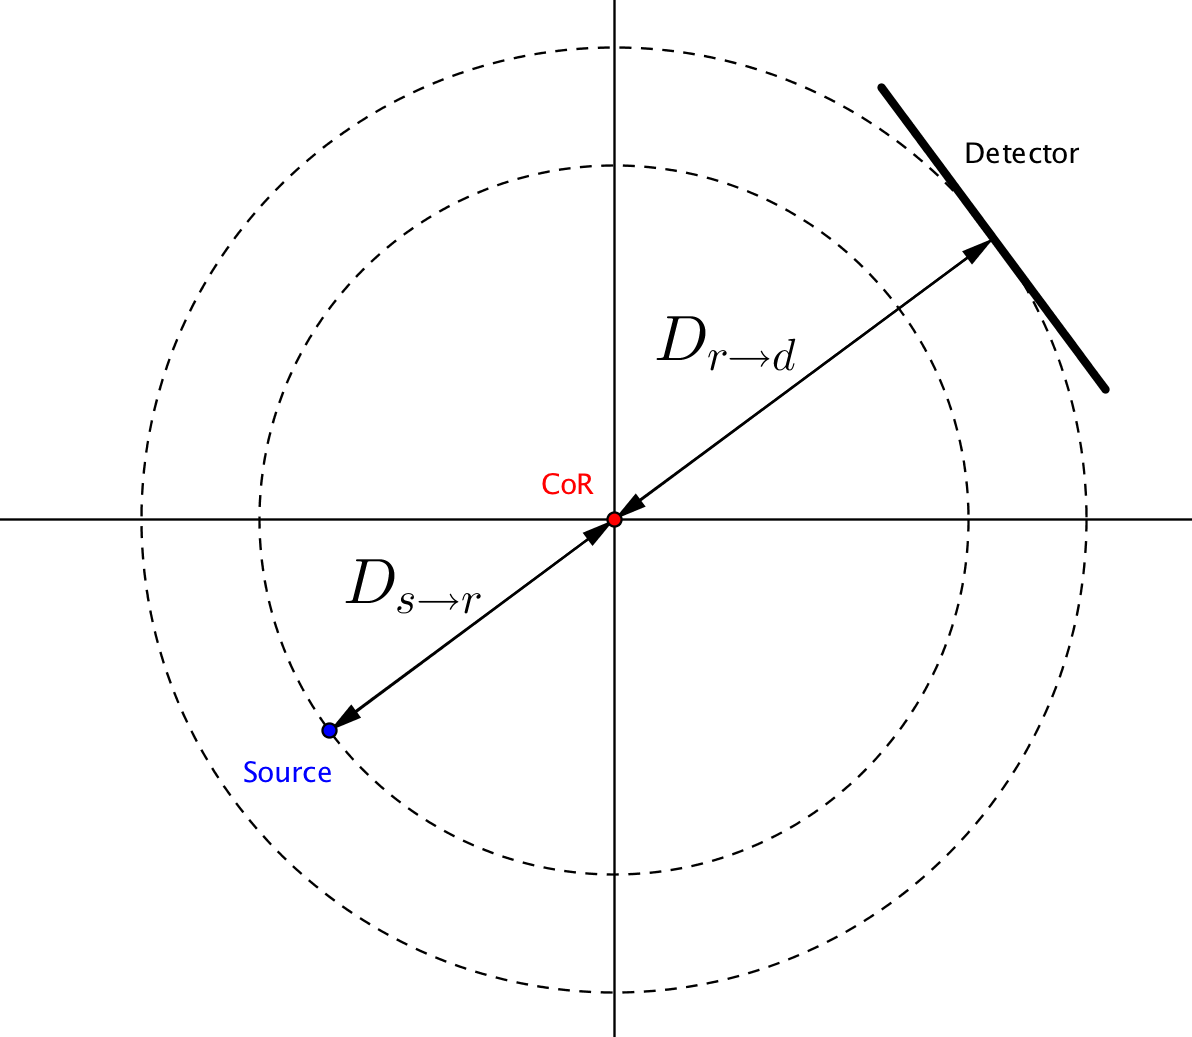
\includegraphics[width=\textwidth]{figures/XCTsystem.png}
    \caption{A digram showing a birds eye view of the XCT system}
    \label{xctsystem}
\end{figure}

\begin{figure}[h!]
  \centering
    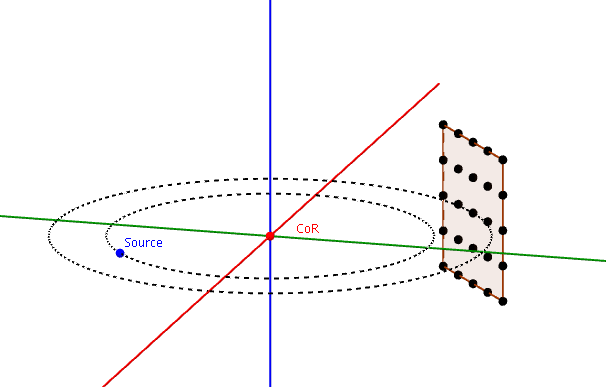
\includegraphics[width=\textwidth]{figures/3dxctsystem.png}
    \caption{A 3D view of the XCT system showing the detector array}
    \label{3dxctsystem}
\end{figure}

In order to simulate more realistic source and detector behavior the projection process is repeated many times at each angle with random offsets applied to the positions of the source and each detector element, the resulting projection values being the mean of the repetitions. In the case of the detector elements this entails adding an independent random offset to each detector element - not the same offset to all.

The experiments undertaken for this project involved the simulation of projections at $1000$ angles between $0$ and $2\pi$. The choice of this particular number of projections was chosen so as maximize the accuracy of the reconstructed volume whilst minimizing computational expense - an investigation of the effect of the number of projections used was not undertaken. The object imaged was a sphere of radius $30mm$ with centre at $c = (0,0,0)^T$. An array of $301\times301$ detector elements was used extending over an area of $400mm\times400mm$. Four experimental treatments were investigated;

\begin{enumerate}
\item $S0D0$ - Ideal point like source and detector elements.
\item $S1D0$ - Random position offset applied to source (each offset drawn from ), point like detector elements.
\item $S0D1$ - Random position offset applied independently to each detector element (each offset drawn from ), point like source.
\item $S1D1$ - Random position offsets applied to both the source and the detector elements (each offset drawn from same distributions as above).
\end{enumerate}

For each treatment projections were simulated at each of $10$ equally spaced magnifications between $1.5$ and $4.0$. At a particular magnification $10$ sets of projections were simulated. This leads to a total of $400$ projections and reconstructions - consisting of four treatments, ten magnifications and ten repetitions at each magnification.






\section{Beam Hardening}
\chapter{Results}

\section{Introduction}

Section in which I outline what will follow in this chapter, also link to previous chapter!

\section{Measurement Uncertainty}

Initially we will look at the average radius, taken over ten repetitions, at each level of magnification. In figure \ref{avgmeasuredradius} we can see the plot of this measurement for each of the four experimental treatments; ideal source and detector ($S0D0$), non-ideal source and ideal detector ($S1D0$), ideal source and non-ideal detector ($S0D1$) and non-ideal source and detector ($S1D1$). As can be seen from the plot all measurements are systematically biased below the true value of the imaged object (30mm). There exist clear trends in the behavior of the measurement as magnification increases for $S1D0$, $S0D1$, and $S1D1$. The ideal imaging system ($S0D0$) exhibits a less clear trend, seeming to be highly noisy.

\begin{figure}[h!]
  \centering
    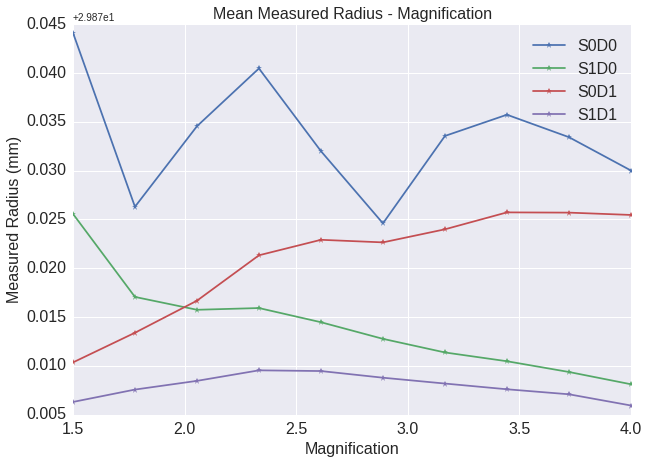
\includegraphics[width=\textwidth]{figures/output_10_0.png}
    \caption{Showing the average radius at each magnification.}
    \label{avgmeasuredradius}
\end{figure}

We can also look at the relative error of the measurements since we are in the position of knowing the true value - this can be seen in figure \ref{relerrormeasuredradius}. The $S0D0$ treatment shows the lowest relative errors of all treatments, there appears to be an increase in the error as magnification increases however the data is rather noisy. Treatments $S1D0$ and $S0D1$ show opposing, possibly linear, trends. Measurements taken with a non-ideal detector seem to get more accurate as magnification increases whereas the measurements taken with a non-ideal source show a decrease in the accuracy with an increase in magnification. When the measurements are taken with both non-ideal source and detector the relative errors are the largest of all treatments. There appears to be a non-linear, perhaps quadratic, relation between magnification and measurement error.

\begin{figure}[h!]
  \centering
    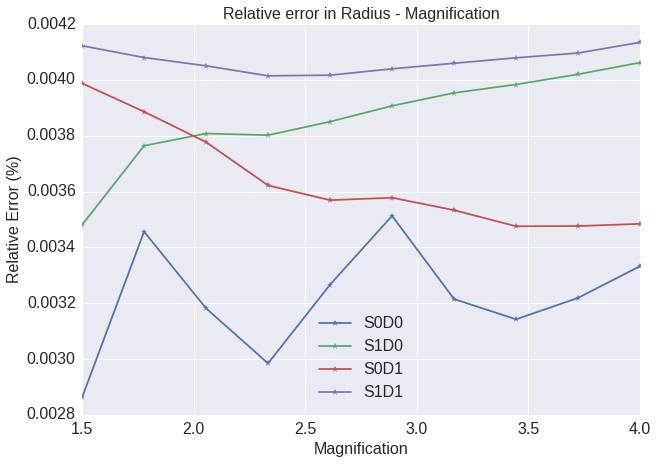
\includegraphics[width=\textwidth]{figures/output_8_0.png}
    \caption{Showing the relative error of the radius measurement at each magnification.}
        \label{relerrormeasuredradius}
\end{figure}

It should be noted that all the measured errors are at the sub-voxel level; the largest error seen is around $0.4\%$ which equates to an actual deviation from the true value of around $0.12$mm less then $2\%$ of the voxel width ($4.2$mm).

In figure \ref{stdmeasuredradius} we can see the variation (standard deviation) in the measurement in relation to magnification. This data is only available for $S1D0$, $S0D1$ and $S1D1$. This is because with an ideal source and detector the measurement is in effect deterministic. The projections do have very small additive noise applied but this is not enough to effect the reconstructions and hence the measurements in any meaningful way.

\begin{figure}[h!]
  \centering
    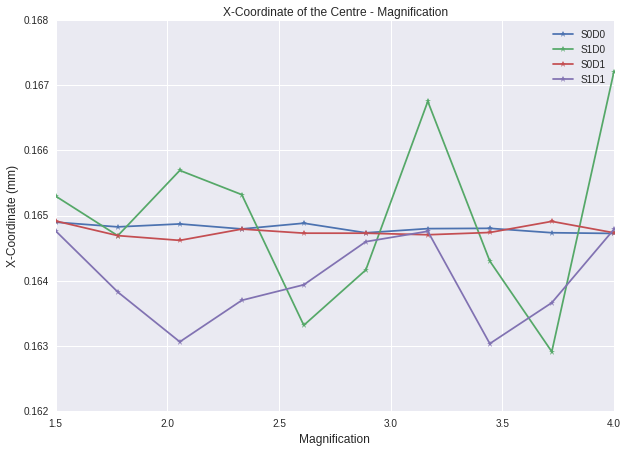
\includegraphics[width=\textwidth]{figures/output_14_0.png}
    \caption{Showing the variation of the radius measurement at each magnification.}
        \label{stdmeasuredradius}
\end{figure}

Any trend in the measurement variation is less clear to see. However if we ignore the data point at a magnification of $1.5$ for $S0D1$ it could be the case that the variation is decreasing with magnification for a non-ideal detector and vice-versa for a non-ideal source. In order to test this hypothesis a further twenty reconstructions were conducted at magnifications of $1.5$, $2.0556$ and $4.0$; the increase in sample size at these points should give a clearer picture of the underlying measurement variation. It would have been of great interest to conduct more reconstructions at all magnifications but this would have taken far too long - the new samples where chosen to cover low, medium and high magnifications in the hope that any trend became clearer. Figure \ref{stdmeasuredradiusxsamples} shows the measurement variation for the higher sampled magnifications. This seems to show that as magnification increases the measurement variability increase for the $S1D0$ treatment and decreases for the the $S0D1$ treatment. In order to further reinforce this conclusion two one tail T-tests where performed to see if the differences in the measurement variation was statistically significant. In the first test, which compares the measurement variance between $S1D0$ and  $S0D1$ at a magnification of $1.5$, the null and alternative hypothesis's are given by;

\[
H_0: \sigma_{S1D0,1.5} = \sigma_{S0D1,1.5}
\]
\[
H_1: \sigma_{S1D0,1.5} < \sigma_{S0D1,1.5}
\]

The test resulted in a test statistic of $F=0.1781$ and p-value of $6.431e-06 < 0.01$ (m=29,n=29 degrees of freedom), so the null hypothesis can be rejected at the 95\% level suggesting that there is significant evidence that $\sigma_{S1D0,1.5} < \sigma_{S0D1,1.5}$. For the second test we will compare the measurement variance between $S1D0$ and  $S0D1$ at a magnification of $4.0$. The null and alternative hypothesis's are given by;

\[
H_0: \sigma_{S1D0,4.0} = \sigma_{S0D1,4.0}
\]
\[
H_1: \sigma_{S1D0,4.0} > \sigma_{S0D1,4.0}
\]

The test resulted in a test statistic $F = 0.1619$ and a p-value of $2.347e-06 < 0.01$ (m=29,n=29 degrees of freedom), so the null hypothesis can be rejected at the 95\% level suggesting that there is significant evidence that $\sigma_{S1D0,4.0} > \sigma_{S0D1,4.0}$.

\begin{figure}[h!]
  \centering
    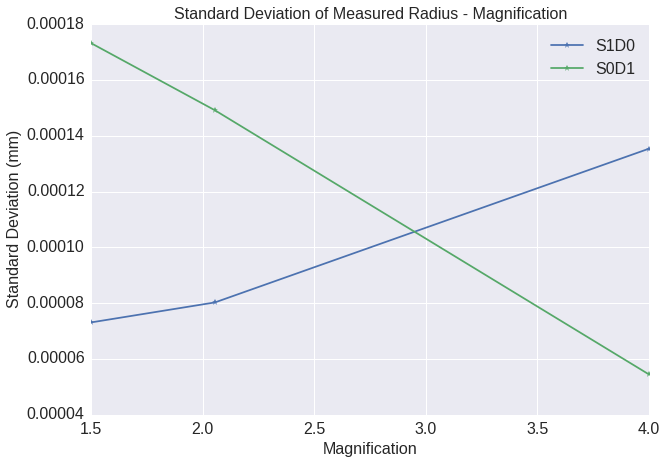
\includegraphics[width=\textwidth]{figures/output_34_0.png}
    \caption{Showing the variation of the radius measurement with a sample of 30 at each magnification.}
        \label{stdmeasuredradiusxsamples}
\end{figure}

The result of the two F-tests reinforces the hypothesis that there exists contrasting trends in measurement uncertainty between $S0D1$ and $S1D0$. It seems clear that an increase in magnification leads to a decrease in measurement variability for $S0D1$ and an increase in the variability for $S1D0$ - with an intersection point (position of equal variability) at a magnification of between $2.5$ and $3.0$. The level of variability in the measurement also relates to the relative error in the measurement; high variability leads to a larger relative error. This can be clearly seen in the error and variability trends of the two treatments $S0D1$ and $S1D0$.

Further to the measurements of the radii, the position of the spheres centers were also calculated. Again all measurements resulted in a systematic bias; figure \ref{spherecentre} shows the average position for a range of magnifications.

\begin{figure}[h!]
  \centering
    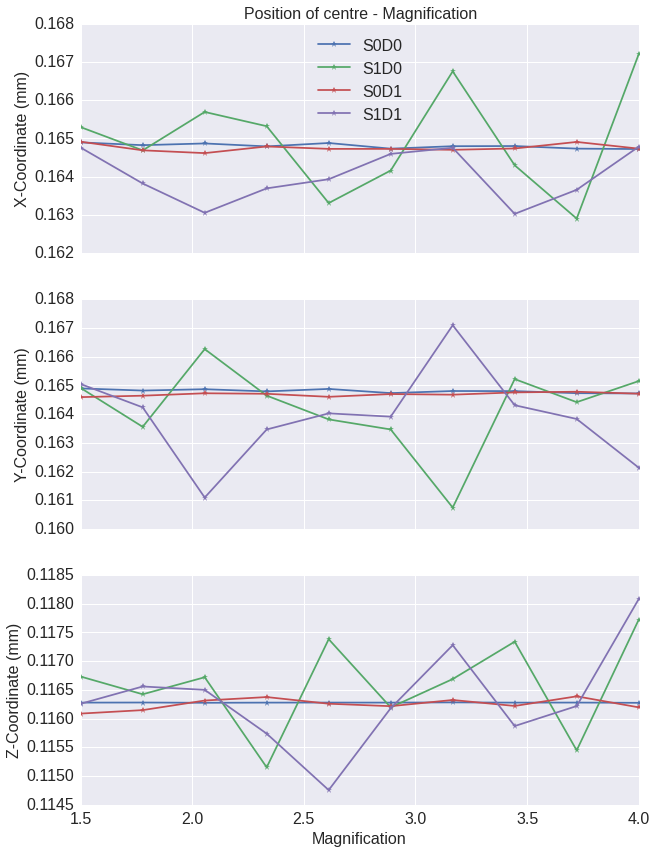
\includegraphics[width=\textwidth]{figures/output_18_0.png}
    \caption{Showing the measured position of the spheres centre}
        \label{spherecentre}
\end{figure}

The average position of the centre does not exhibit any clear trend with respect to magnification. There does however seem to be differences between the individual treatments. Both $S0D0$ and $S0D1$ show little variation in the measured position as magnification varies, whereas $S1D1$ and $S1D0$ exhibit much greater fluctuations in the measured position. The standard deviation of the measured position, taken over ten repetitions at each magnification, is shown in figure \ref{spherecentrevar}. The logarithmic plot shows that the variation is an order of magnitude larger for $S1D0$ and $S1D1$ than for $S0D1$. This contrasts with the variation in the measured radius for which the standard deviation was approximately of the same magnitude for both $S1D0$ and $S0D1$.

\begin{figure}[h!]
  \centering
    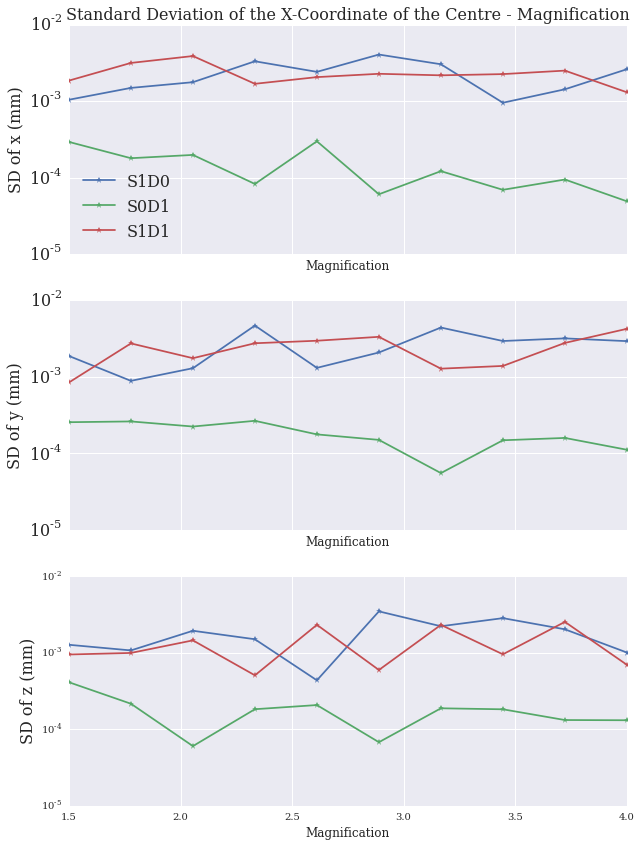
\includegraphics[width=\textwidth]{figures/output_22_0.png}
    \caption{Showing the standard deviation of the measured position of the spheres centre}
        \label{spherecentrevar}
\end{figure}

\section{Polychromatic Projections}

\section{Image Resolution}

\section{Analytic MTF}


\chapter{Conclusion}




\end{document}
